% Standalone supplementary-figure manuscript for the authenticated F29R7 study.
% Compile ONLY after generating PDF graphics using
% plot_f29r7_legacy_style_from_verified_results.py on the actual WSL files.
% This is not part of the original 24 primary-hypothesis family.
\documentclass[11pt,a4paper]{article}
\usepackage[margin=25mm]{geometry}
\usepackage{graphicx}
\usepackage{caption}
\usepackage{hyperref}
\graphicspath{{F29R7_Style_Recreations_Supplementary/}}
\renewcommand{\thefigure}{S\arabic{figure}}
\begin{document}
\begin{center}
{\Large\bfseries Supplementary Figures}\par\medskip
{\large Leakage-Controlled Multi-Horizon Directional Forecasting of Indian Equities}\par
\end{center}

\noindent\textbf{Evidence scope.} All plotted scores derive from the authenticated F29R7 amended held-out sample of 5,300 equity-session endpoints on 265 trading sessions. The plots are descriptive and exploratory; the original confirmatory inference is restricted to 24 neural architecture--horizon balanced-accuracy hypotheses. No new training, test access, inference, or bootstrap recomputation was performed to generate these figures.

\begin{figure}[p]
\centering
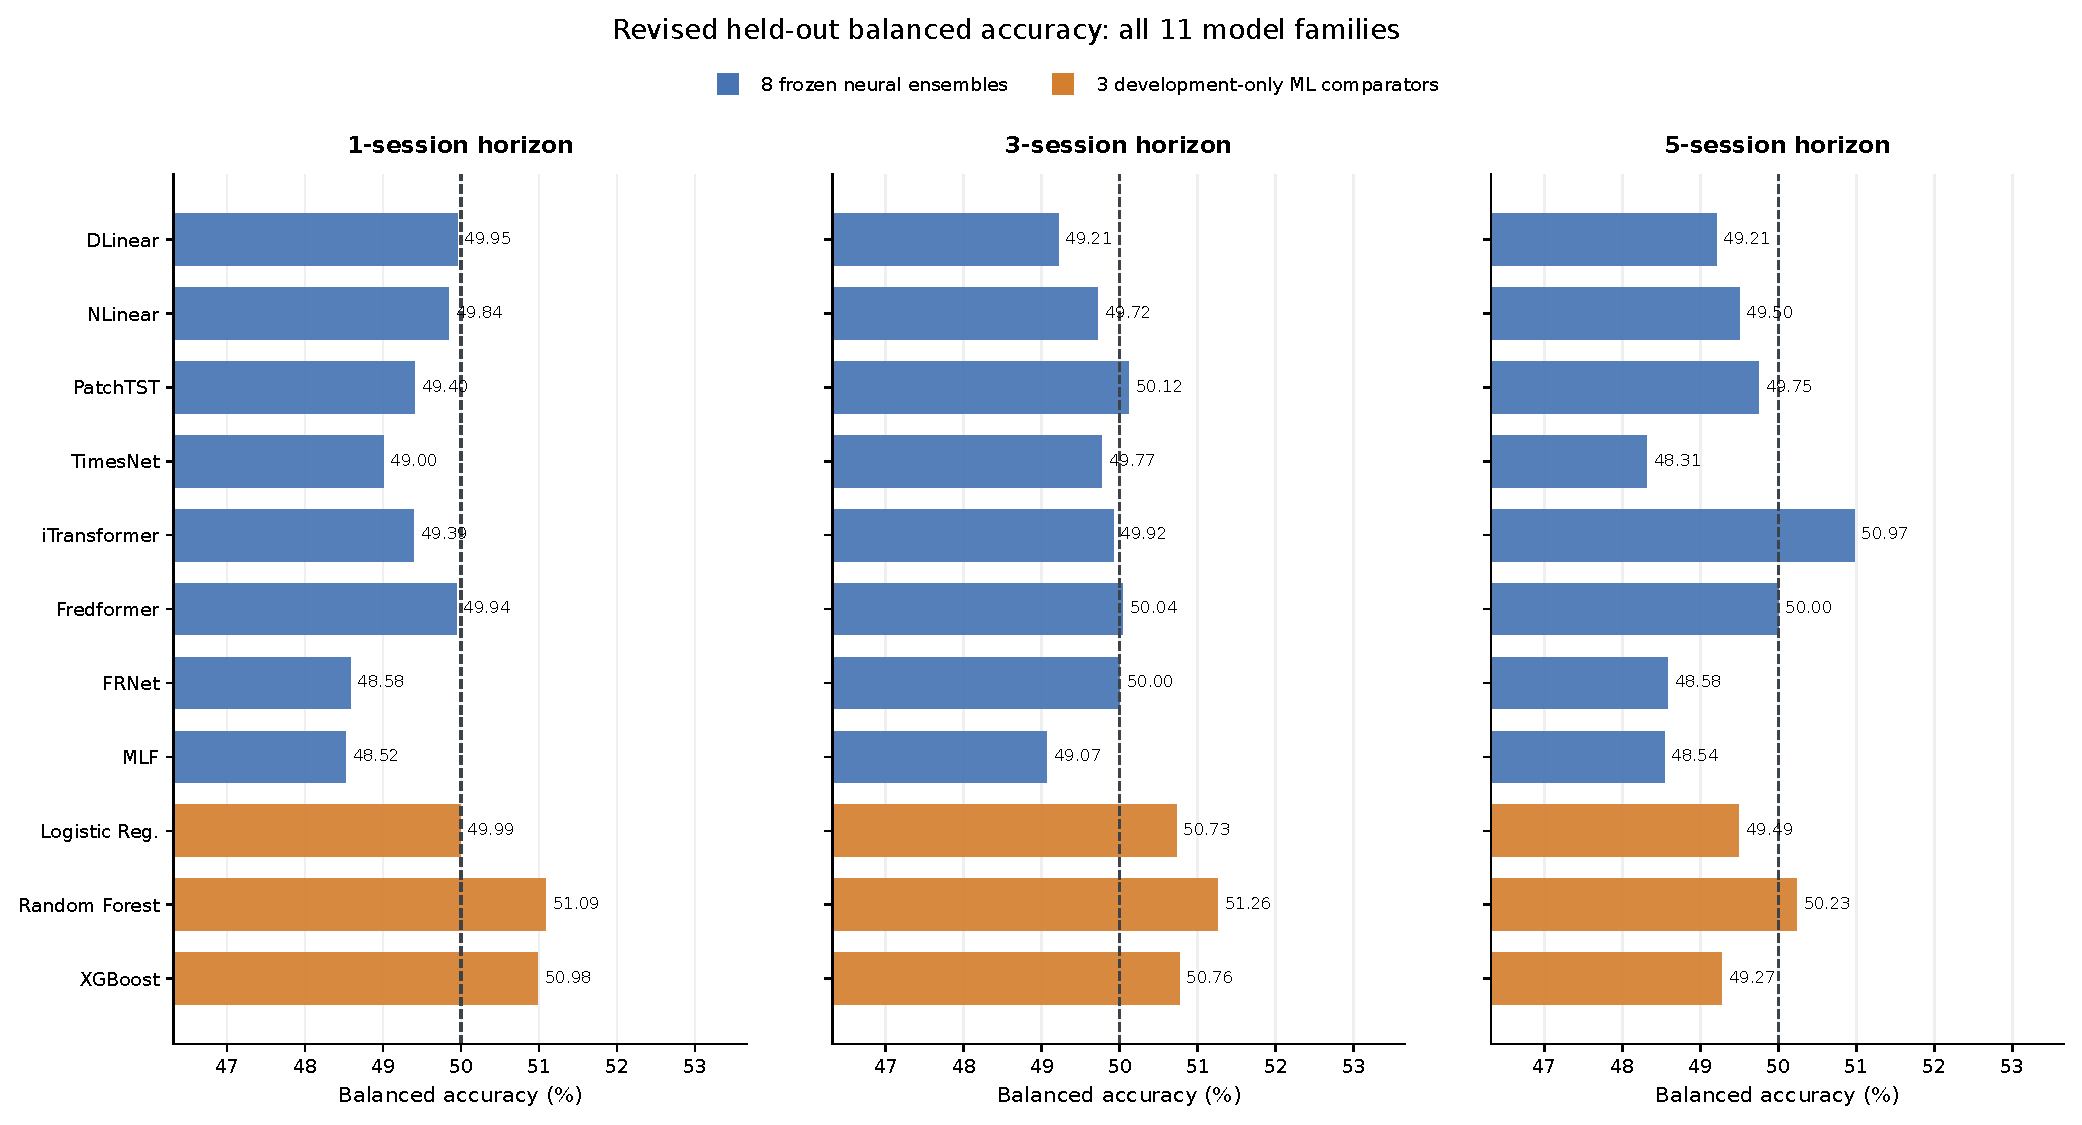
\includegraphics[width=\textwidth]{sup01_all_neural_ml_BA_bars.pdf}
\caption{Balanced accuracy of all eight frozen five-seed neural ensembles and three development-trained conventional ML comparators at one-, three-, and five-session horizons. Each estimate uses the identical 5,300 endpoint cohort. The dashed line denotes balanced accuracy of 50\%. Conventional ML comparisons are exploratory and these bars do not demonstrate statistical superiority.}
\label{fig:sup_ba_bars}
\end{figure}
\begin{figure}[p]
\centering
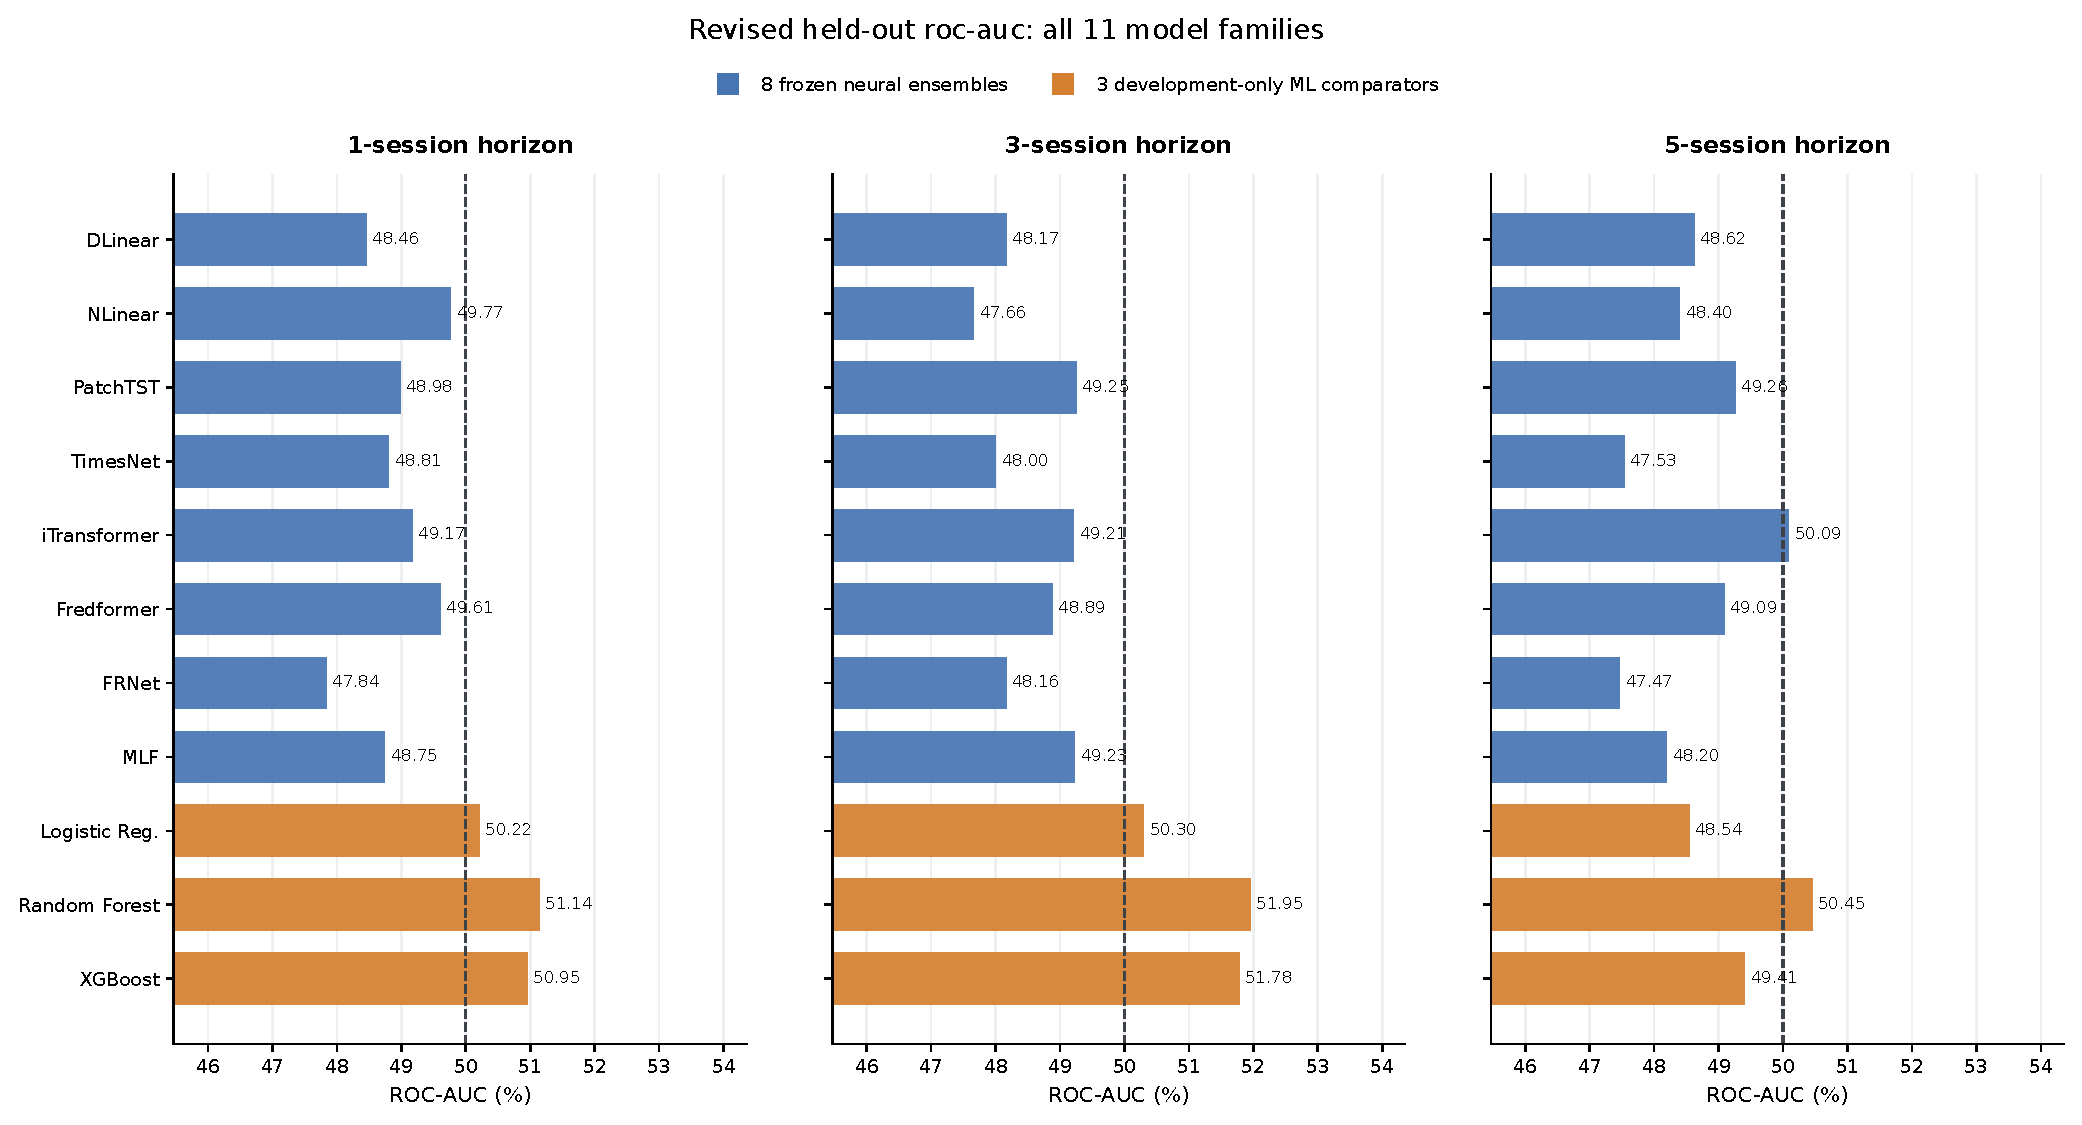
\includegraphics[width=\textwidth]{sup02_all_neural_ml_ROCAUC_bars.pdf}
\caption{Descriptive ROC-AUC scores for the eleven model families at the three forecasting horizons. Values are authenticated point estimates; this figure deliberately does not show uncomputed ROC-AUC confidence intervals. Model families use their original frozen inference rules.}
\label{fig:sup_auc_bars}
\end{figure}
\begin{figure}[p]
\centering
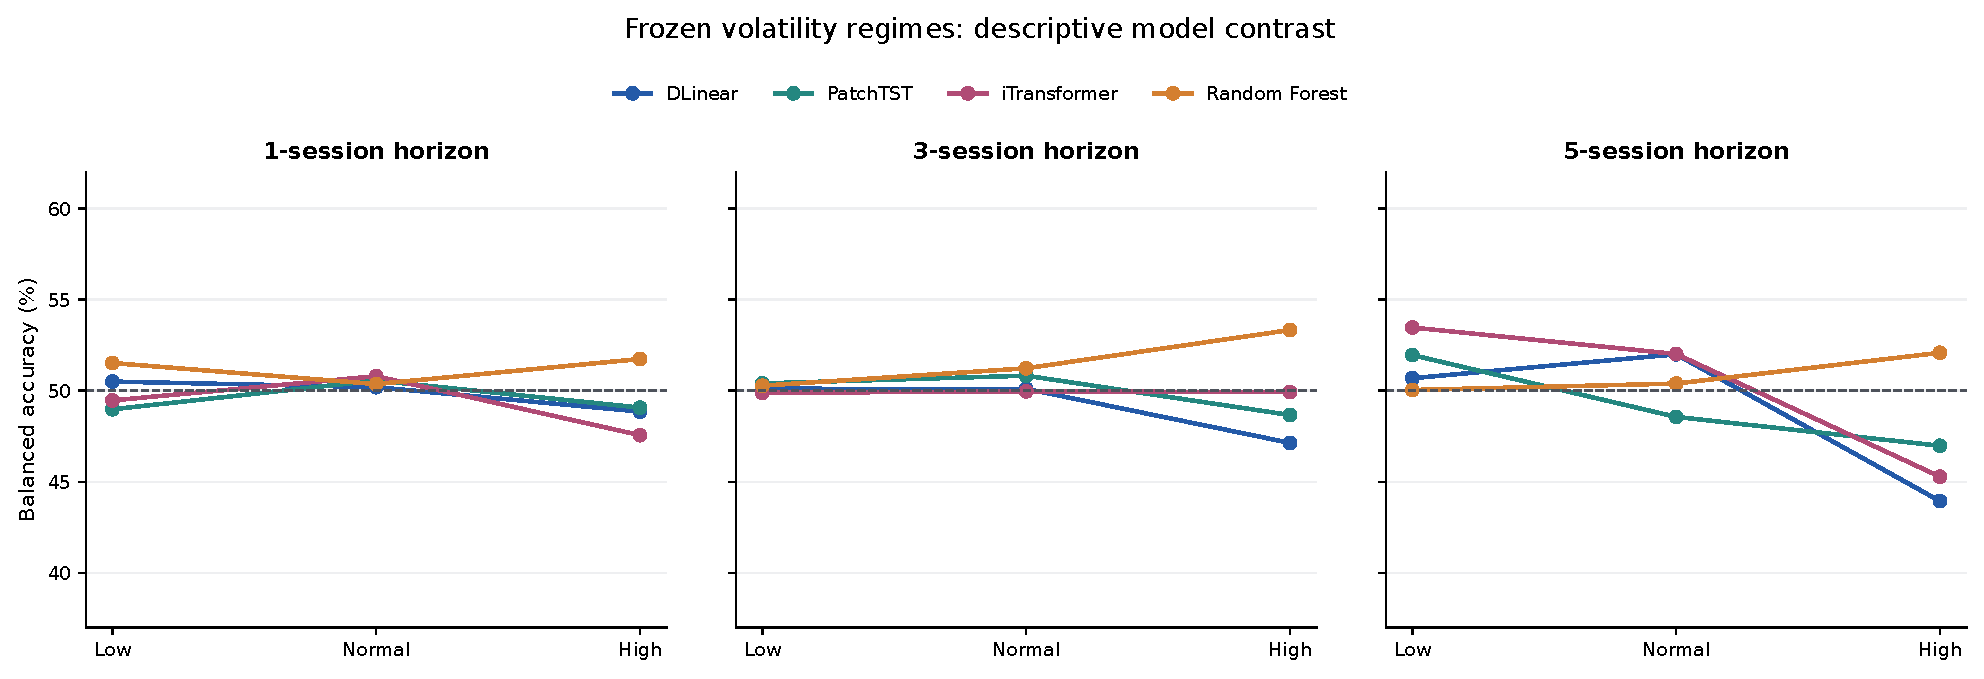
\includegraphics[width=\textwidth]{sup03_regimes_by_horizon.pdf}
\caption{Exploratory model- and horizon-specific balanced accuracy across the frozen Low, Normal, and High volatility regimes. DLinear, PatchTST, iTransformer, and Random Forest are displayed for visual comparability. Lines connect ordered categorical regime summaries \emph{within} a horizon for visual guidance only, not as evidence of continuity, a significant interaction, or a profitable regime-selection strategy.}
\label{fig:sup_regimes}
\end{figure}
\begin{figure}[p]
\centering
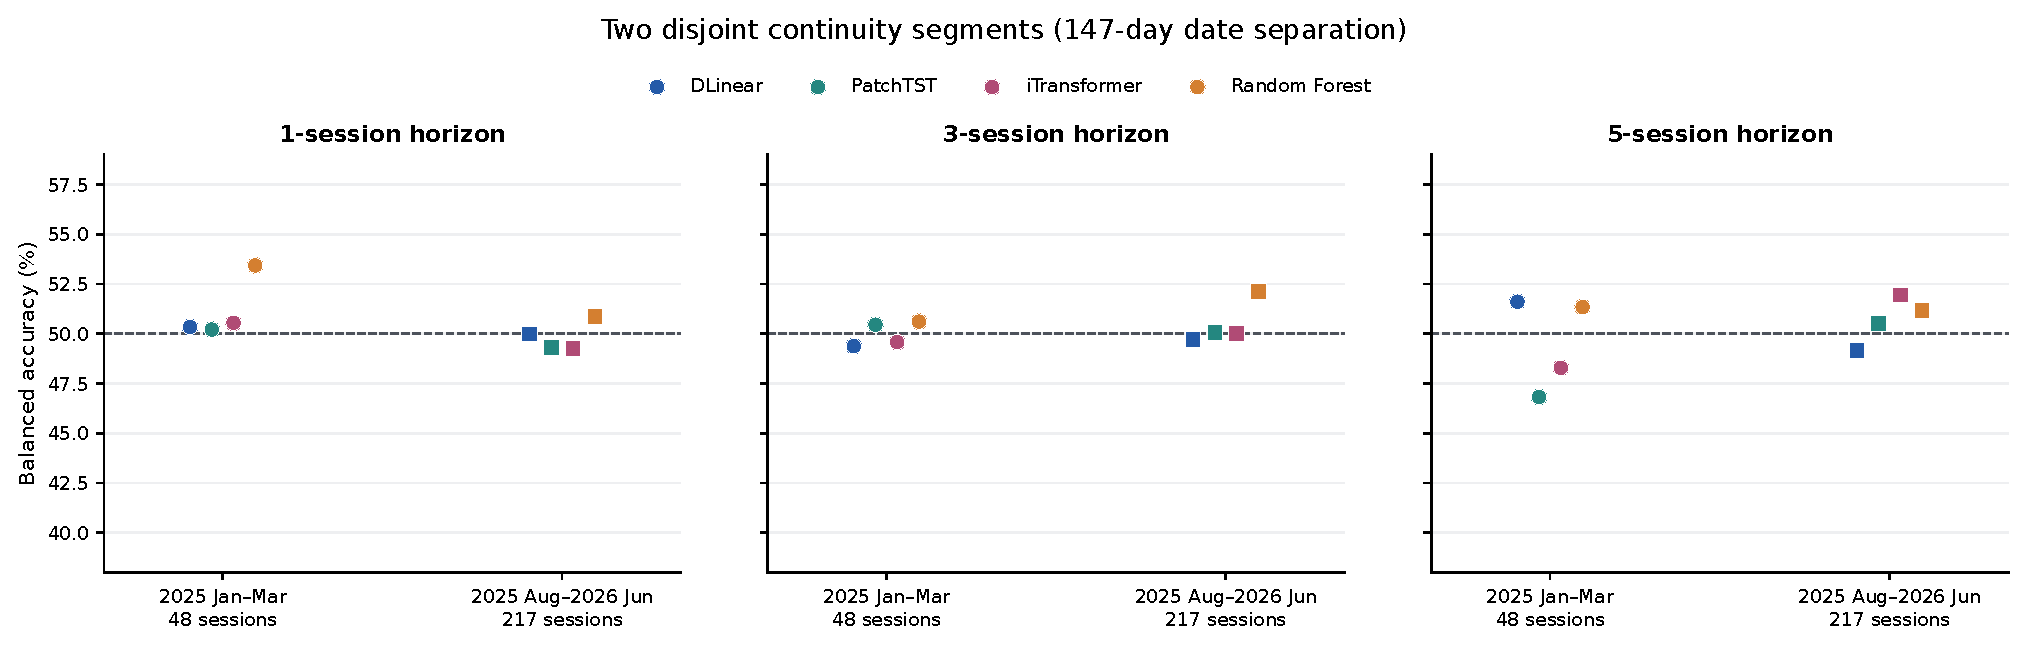
\includegraphics[width=\textwidth]{sup04_disjoint_segment_stability.pdf}
\caption{Exploratory balanced accuracy by the two verified, nonadjacent final-test continuity segments: 48 sessions (960 endpoints) from 1 January to 7 March 2025, and 217 sessions (4,340 endpoints) from 1 August 2025 to 22 June 2026. Disconnected markers explicitly avoid implying continuity across the 147-calendar-day separation.}
\label{fig:sup_segments}
\end{figure}
\begin{figure}[p]
\centering
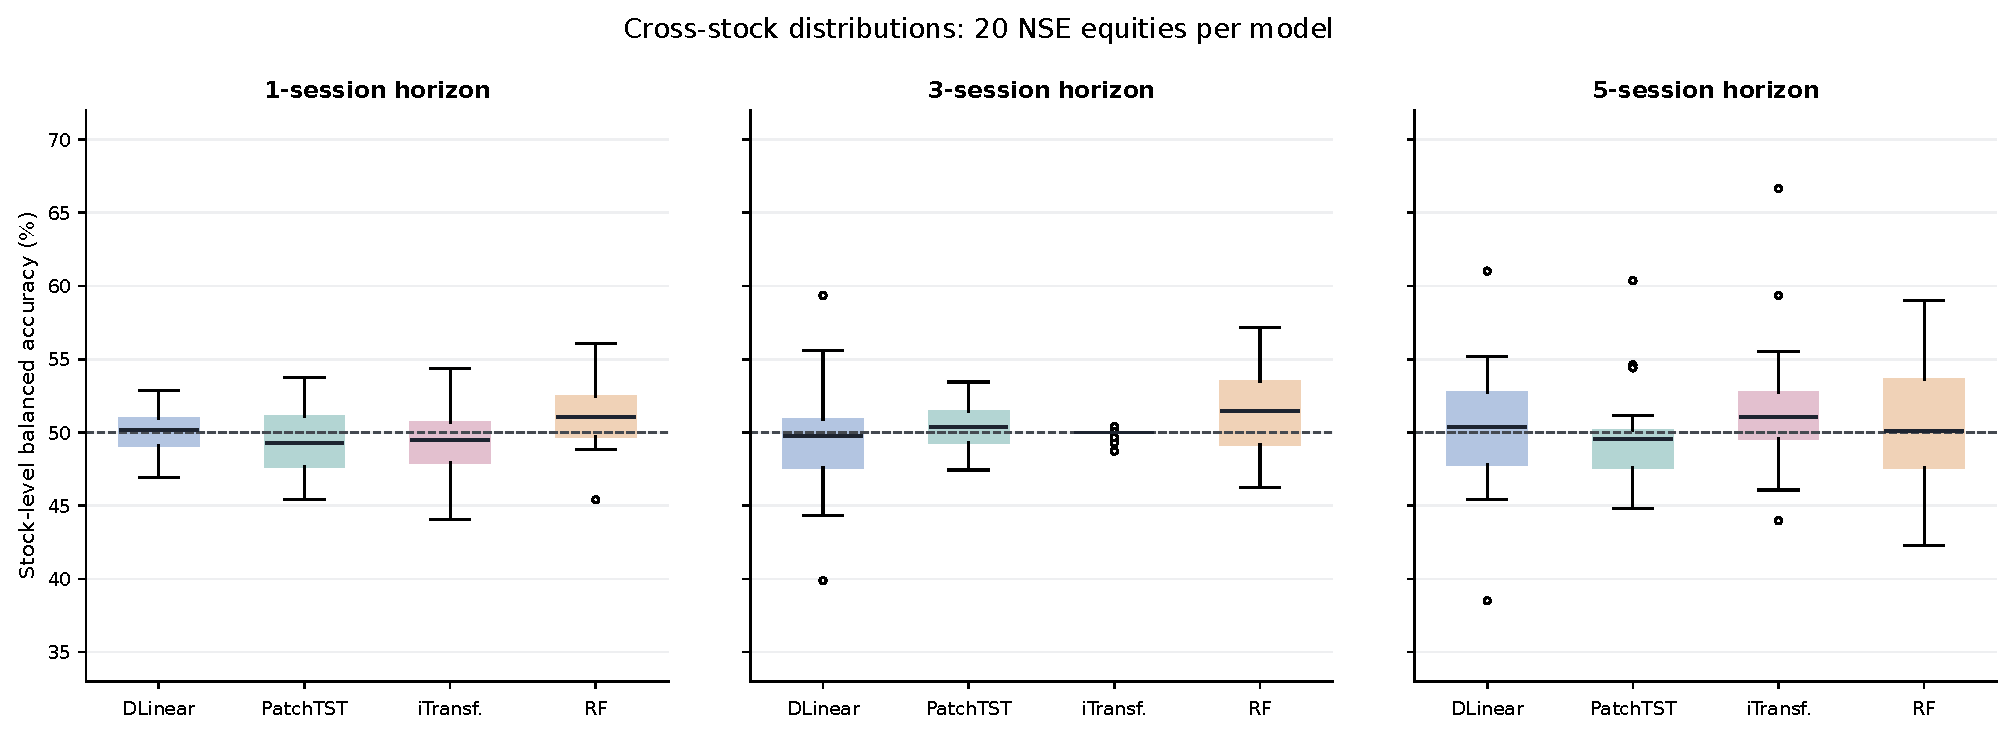
\includegraphics[width=\textwidth]{sup05_stock_level_BA_boxplots.pdf}
\caption{Cross-sectional distribution of stock-level balanced accuracy for four displayed model families across the one-, three-, and five-session tasks. Each box summarizes twenty held-out equities (265 endpoints per equity); whiskers use the Tukey 1.5-IQR convention. Descriptive variation is not a prospective stock-selection policy.}
\label{fig:sup_stock_boxplots}
\end{figure}
\begin{figure}[p]
\centering
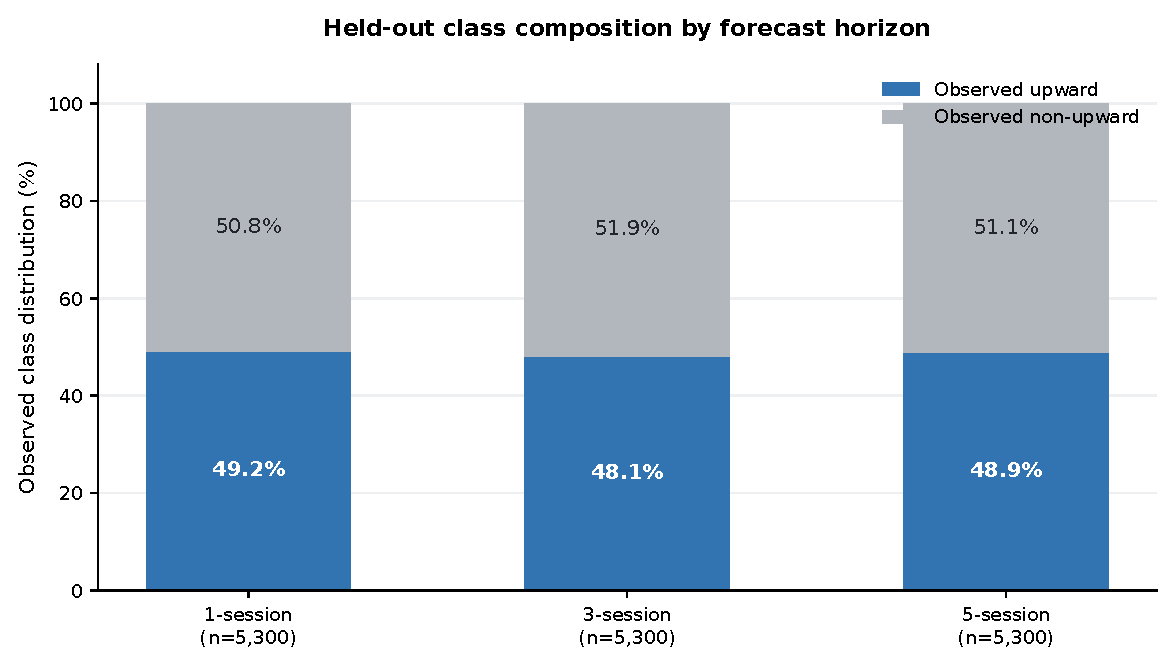
\includegraphics[width=.81\textwidth]{sup06_heldout_up_class_balance.pdf}
\caption{Observed upward and non-upward target-class proportions at each forecasting horizon within the same amended held-out cohort. The values are derived from authenticated confusion-matrix totals. This is \emph{not} a training/validation/test composition plot.}
\label{fig:sup_heldout_classes}
\end{figure}
\begin{figure}[p]
\centering
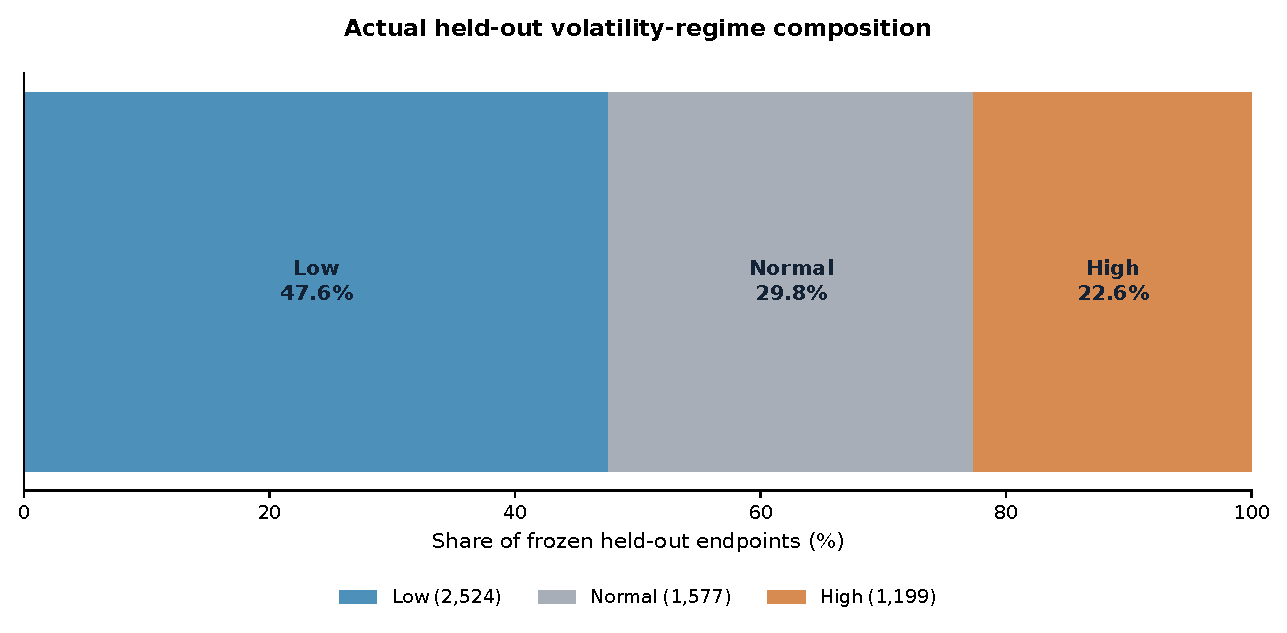
\includegraphics[width=.85\textwidth]{sup07_heldout_regime_composition.pdf}
\caption{Frozen volatility-regime composition of the 5,300 amended held-out observations (Low: 2,524; Normal: 1,577; High: 1,199). The graph does not claim that these were the proportions in training or validation.}
\label{fig:sup_heldout_regimes}
\end{figure}
\clearpage
\end{document}
